% Chapter 5

\chapter{Construction of the Straw Tracking detectors} % Main chapter title

\label{Chapter5} % For referencing the chapter elsewhere, use \ref{Chapter5} 

\section{Introduction}

This chapter will give details on the construction of the E989 straw tracking detectors as described in Chapter 5. This includes each step in the construction process and the strict quality control tests which were meticulously carried out after each of these steps. This was done to ensure that the tracker modules run effectively and meet the design specifications required by the Technical Design Report (TDR)\cite{Reference29}.

The straw tracking detectors were constructed by University of Liverpool staff and students in the ISO Class 5 cleanroom. This was done to prevent any contaminants from entering the module during construction. A total of 22 modules were produced and tested in Liverpool before being shipped to Fermilab. 

\section{Pre-assembly checks and preparation}

Before construction can be started a series of checks and preparations must be carried out prior to beginning construction of a tracking module. The gold-plated copper pins which fix the wire in place within the manifold must be cleaned for any blockages inside before they can be used to construct wires. This is done by placing the pins in an ultrasonic cleaner which uses de-ionized water and then secondly cleaned with isopropanol alcohol. Once the pins have dried, any remaining blockages can be removed by threading the pins with thicker 50 $\mu$m gold-plated tungsten wire. The Aluminized Mylar straws are also visually inspected for any observable damage, kinks or unravelling of the straws that would lead to gas leakage. These straws are not passed onto the next stage of construction. 

The straws are measured and should all be approximately 1.3 m long and 5 mm in diameter. The electrical resistance is measured before and after the supportive inner layer of paper is removed from the straw. If the resistance changes dramatically after the removal of the paper, this would indicate that damage has been created when removing it. The resistance for each straw should be around 200$\Omega$ for both measurements. Any straw with a much higher or lower value or a straw with a changing resistance will not be used in the construction process. The straws that pass will then be prepared for a leak test. 

\subsection {Leak testing}

The rate of permeation of $CO_{2}$ that flows through the straw wall is calculated for every straw. Only the straws with the lowest permeation rates and do not exceed the leak rate specified by the TDR will be selected for module construction. As the Mylar straws are known to be permeable to some gases it was predicted that some gas leakage would be present. The experiment is operated under vacuum and in order for the quadrupoles to operate at the required voltage the Storage Ring vacuum cannot exceed $10^{-6}$ Torr. In order to achieve this each tracker station must have a maximum leak rate of $4.5\times10^{-5}$ Torr·L/s, therefore each tracking module must not exceed $5.6\times10^{-6}$ Torr·L/s. Anything above this is too high to be handled by the Storage Ring pumping system.

\begin{figure}[h]
\centering
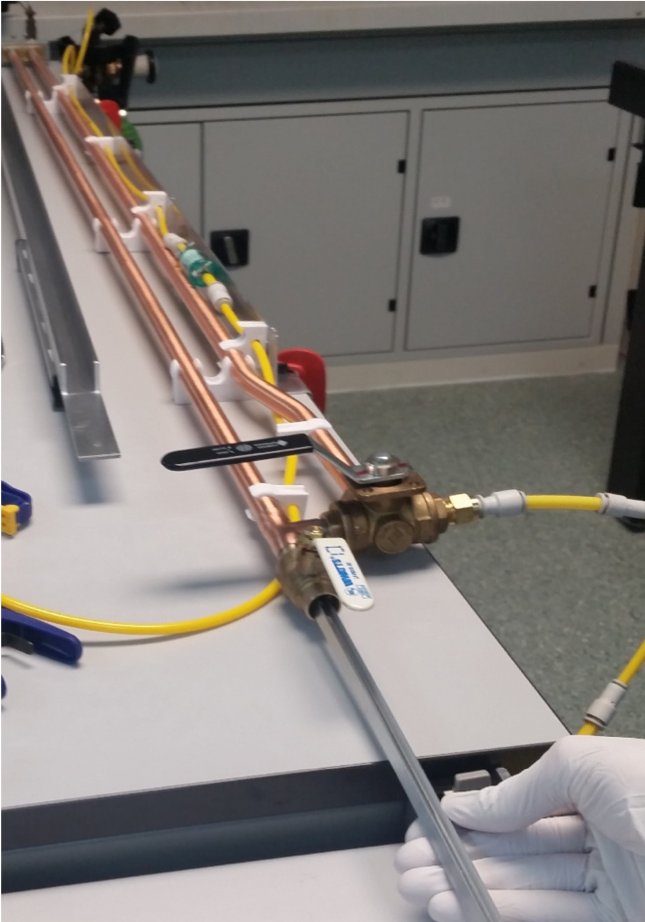
\includegraphics[scale=0.8]{Figures/leaktestsetup}
\decoRule
\caption{Photograph of a straw being placed into the leak testing equipment}
\label{fig:leaktestsetup}
\end{figure}

The leak tests were done using $CO_{2}$ rather than the experimental gas mixture of 50:50 $Ar:C_{2}H_{6}$ as this was not available for use in the University of Liverpool cleanroom. The leak rate measured is then converted to $Ar:C_{2}H_{6}$ to determine if the straws have a low enough permeation rate to be used in the experiment. The chamber for testing the permeation rate is constructed from Copper pipes and was designed by members of the Mu2e experiment. A photograph of the setup is shown in figure 6.1. This chamber will hold a Nitrogen environment while a straw is placed inside and includes a $CO_{2}$ sensor. The method of the leak testing begins by flushing the test chamber with Nitrogen to remove any other gases present in the chamber. Whilst this is taking place the straws are flushed with $CO_{2}$ to clear out any other gases within the straws. This is done by gluing a gas inlet of Viton tubing to each end of the straw. The gas line to the $CO_{2}$ is then attached to one end to flow the gas through the straw. This is done for one minute. Then the end furthest from the gas line is sealed to allow the straw to fill up with $CO_{2}$. Initially this is over pressured to 1.7 relative to Atm. This is to ensure that the straws will easily be able to cope with the experimental vacuum of 1 Atm. The gas pressure is then reduced to 1 Atm relative and filled at a rate of 0.15 LPM. While this is occurring the straw is inspected for any leaks. The straw is then sealed off from the flow of $CO_{2}$ and further inspected for any deflation of the straw due to holes. The straw is then immediately placed into the test chamber which is then sealed shut. Ensuring that the straw is not kinked or bent at all throughout the testing process to minimise the risk of damage to the straw. Within the test chamber, the $CO_{2}$ sensor records the levels of $CO_{2}$ that passes through the straw wall into the test chamber. This test is carried out for 40 minutes with the $CO_{2}$ level as a function of time displayed. The leak rate is calculated as a slope of this distribution as shown in figure 6.2. There were two separate batches of straws tested throughout the construction process. During pre-testing preparation it was discovered that the PPG4 straws had a wall thickness of 13$\mu$m, which is 2$\mu$m less than batch PPG3. Due to the concern that the PPG4 straws would have a much larger permeation rate and therefore a larger failure rate studies were carried out to see if the maximum leak rate for the PPG4 straws could be increased and still be under the required leak rate. To keep within design specifications the final leak rates allowed were a maximum leak rate of $20\times10^{-5}$cc/min for the PPG3 straws and $40\times10^{-5}$cc/min for the PPG4 straws. The pass rates for all PPG3 straws was 88$\%$ and 86$\%$ for all PPG4 straws.

\begin{figure}[th]
\centering
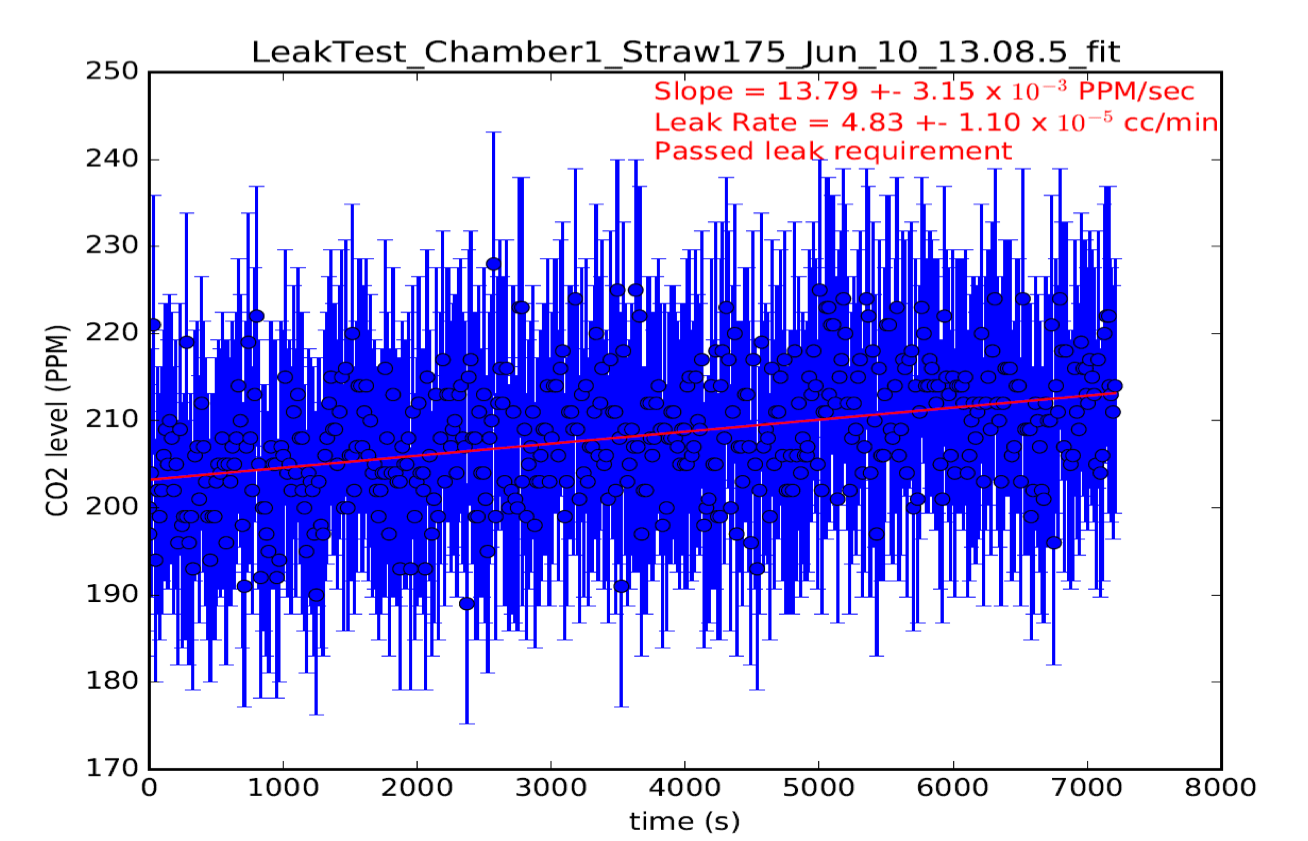
\includegraphics[scale=0.7]{Figures/leaktestplot}
\decoRule
\caption{Graph of a straw with a passed leak rate of $4.83\times10^{-5}cc/min$}
\label{fig:leaktestplot}
\end{figure}

\subsection {Pre-installation ASDQ testing}

Prior to installation each ASDQ board was tested to ensure that the readout electronics and all 16 channels per ASDQ board were working correctly. This involves a setup where each ASDQ is connected by Kapton flexi-cables to a set of  secondary electronics as would be done in the actual experimental setup, shown in figure 6.3. Instead of using muon cosmic data which is used in a later stage of module testing, pulses are sent to the ASDQ. Here 20 pulses are sent to each of the ASDQ’s 16 channels, where the leading edge and the trailing edge are counted. If the channel is working correctly all the pulses should be sent back and so 40 hits will be read per channel. A plot of an ASQD working correctly is shown in figure 6.4. An example of an ASDQ with connection problems is shown in figure 6.5. Out of 165 ASDQs tested, 24 failed giving a pass rate of 85.5$\%$.
\begin{figure}[th]
\centering
\includegraphics[scale=0.3]{Figures/ASDQtestSetup}
\decoRule
\caption{Photograph of testing two ASDQ boards with the ASDQ testing setup}
\label{fig:ASDQtestSetup}
\end{figure}

\newpage
\vfill
\begin{figure}[th]
\centering
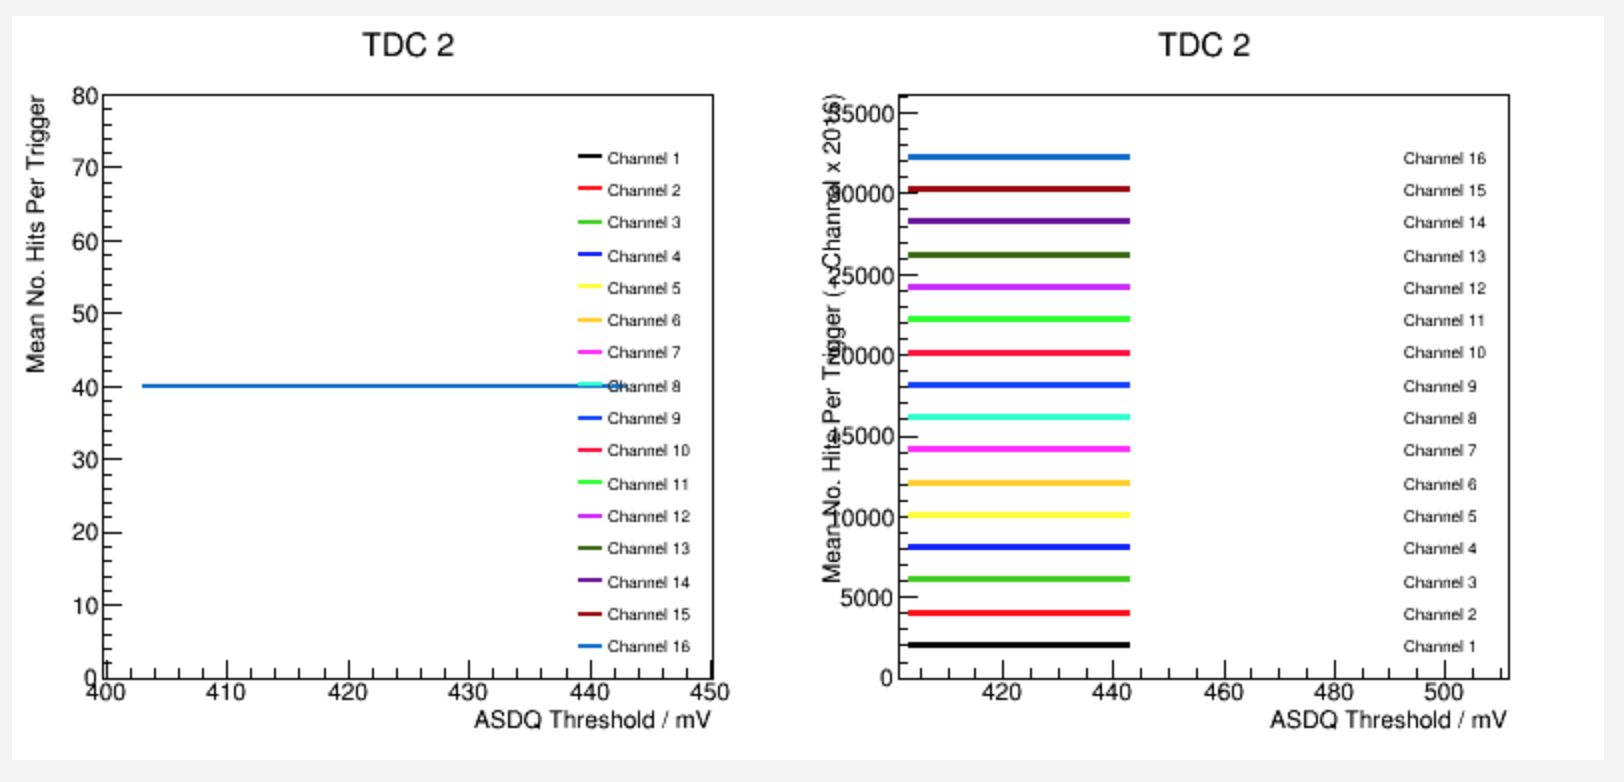
\includegraphics[scale=0.5]{Figures/asdq_testing1}
\decoRule
\caption{Example plot of an ASDQ that has passed testing with all channels recording 40 hits.}
\label{fig:asdq_testing1}
\end{figure}

\begin{figure}[th]
\centering
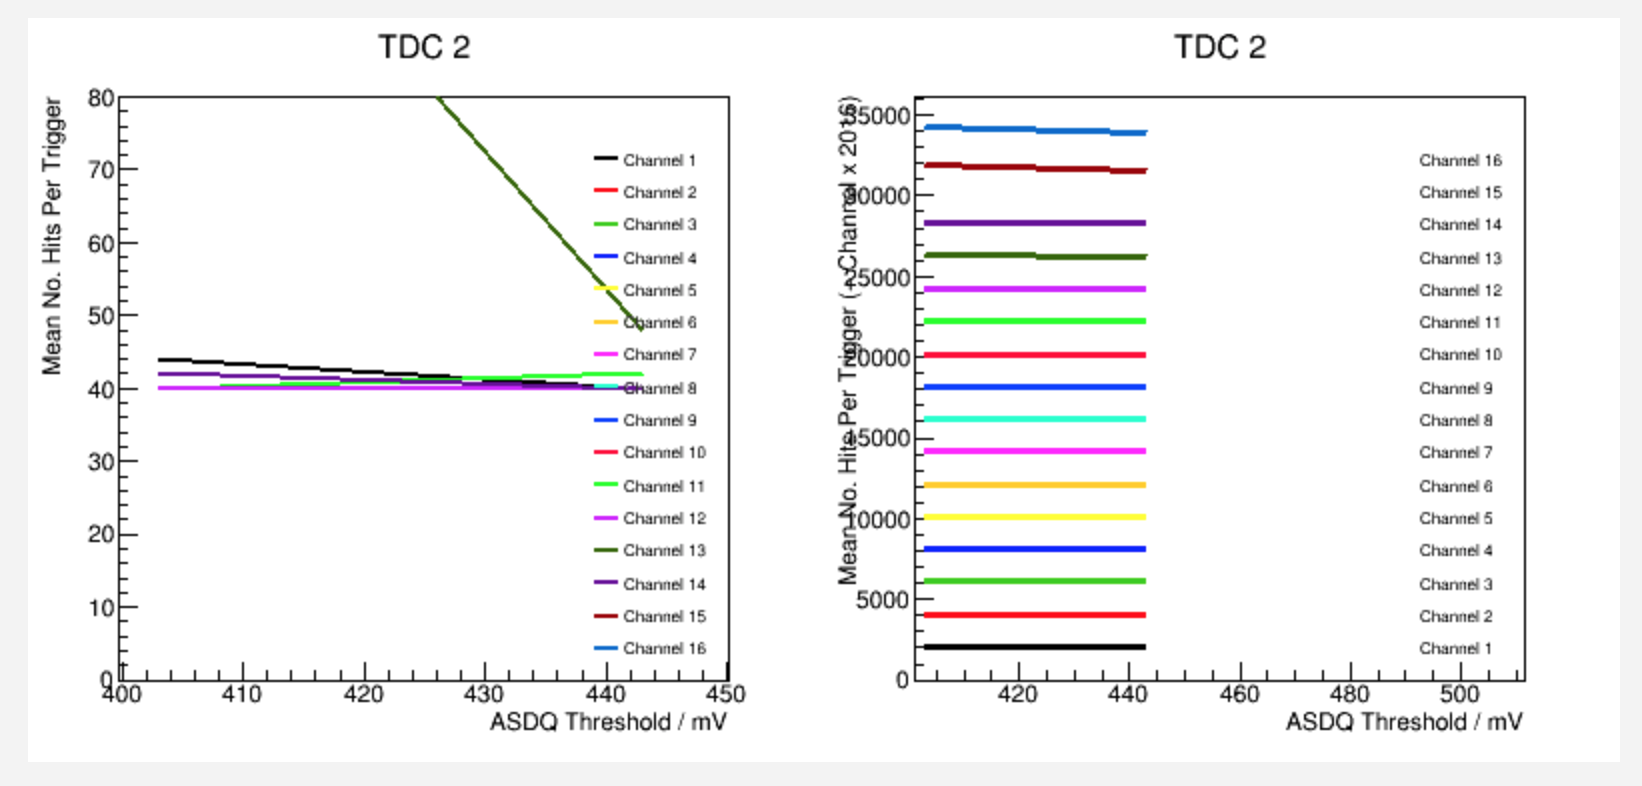
\includegraphics[scale=0.5]{Figures/asdq_testing2}
\decoRule
\caption{Example plot of an ASDQ that has failed testing. This shows that there are several noisy channels producing more than 40 hits.}
\label{fig:asdq_testing2}
\end{figure}
\vfill
\clearpage

\section{Metrology}

Before assembly, the manifolds, flanges and lids are metrology tested. This is to determine the flatness, any tilts of the pieces, along with any wrongly sized or positioned holes. The information is also used to match together two manifolds and a flange for every module. 

\begin{figure}[th]
\centering
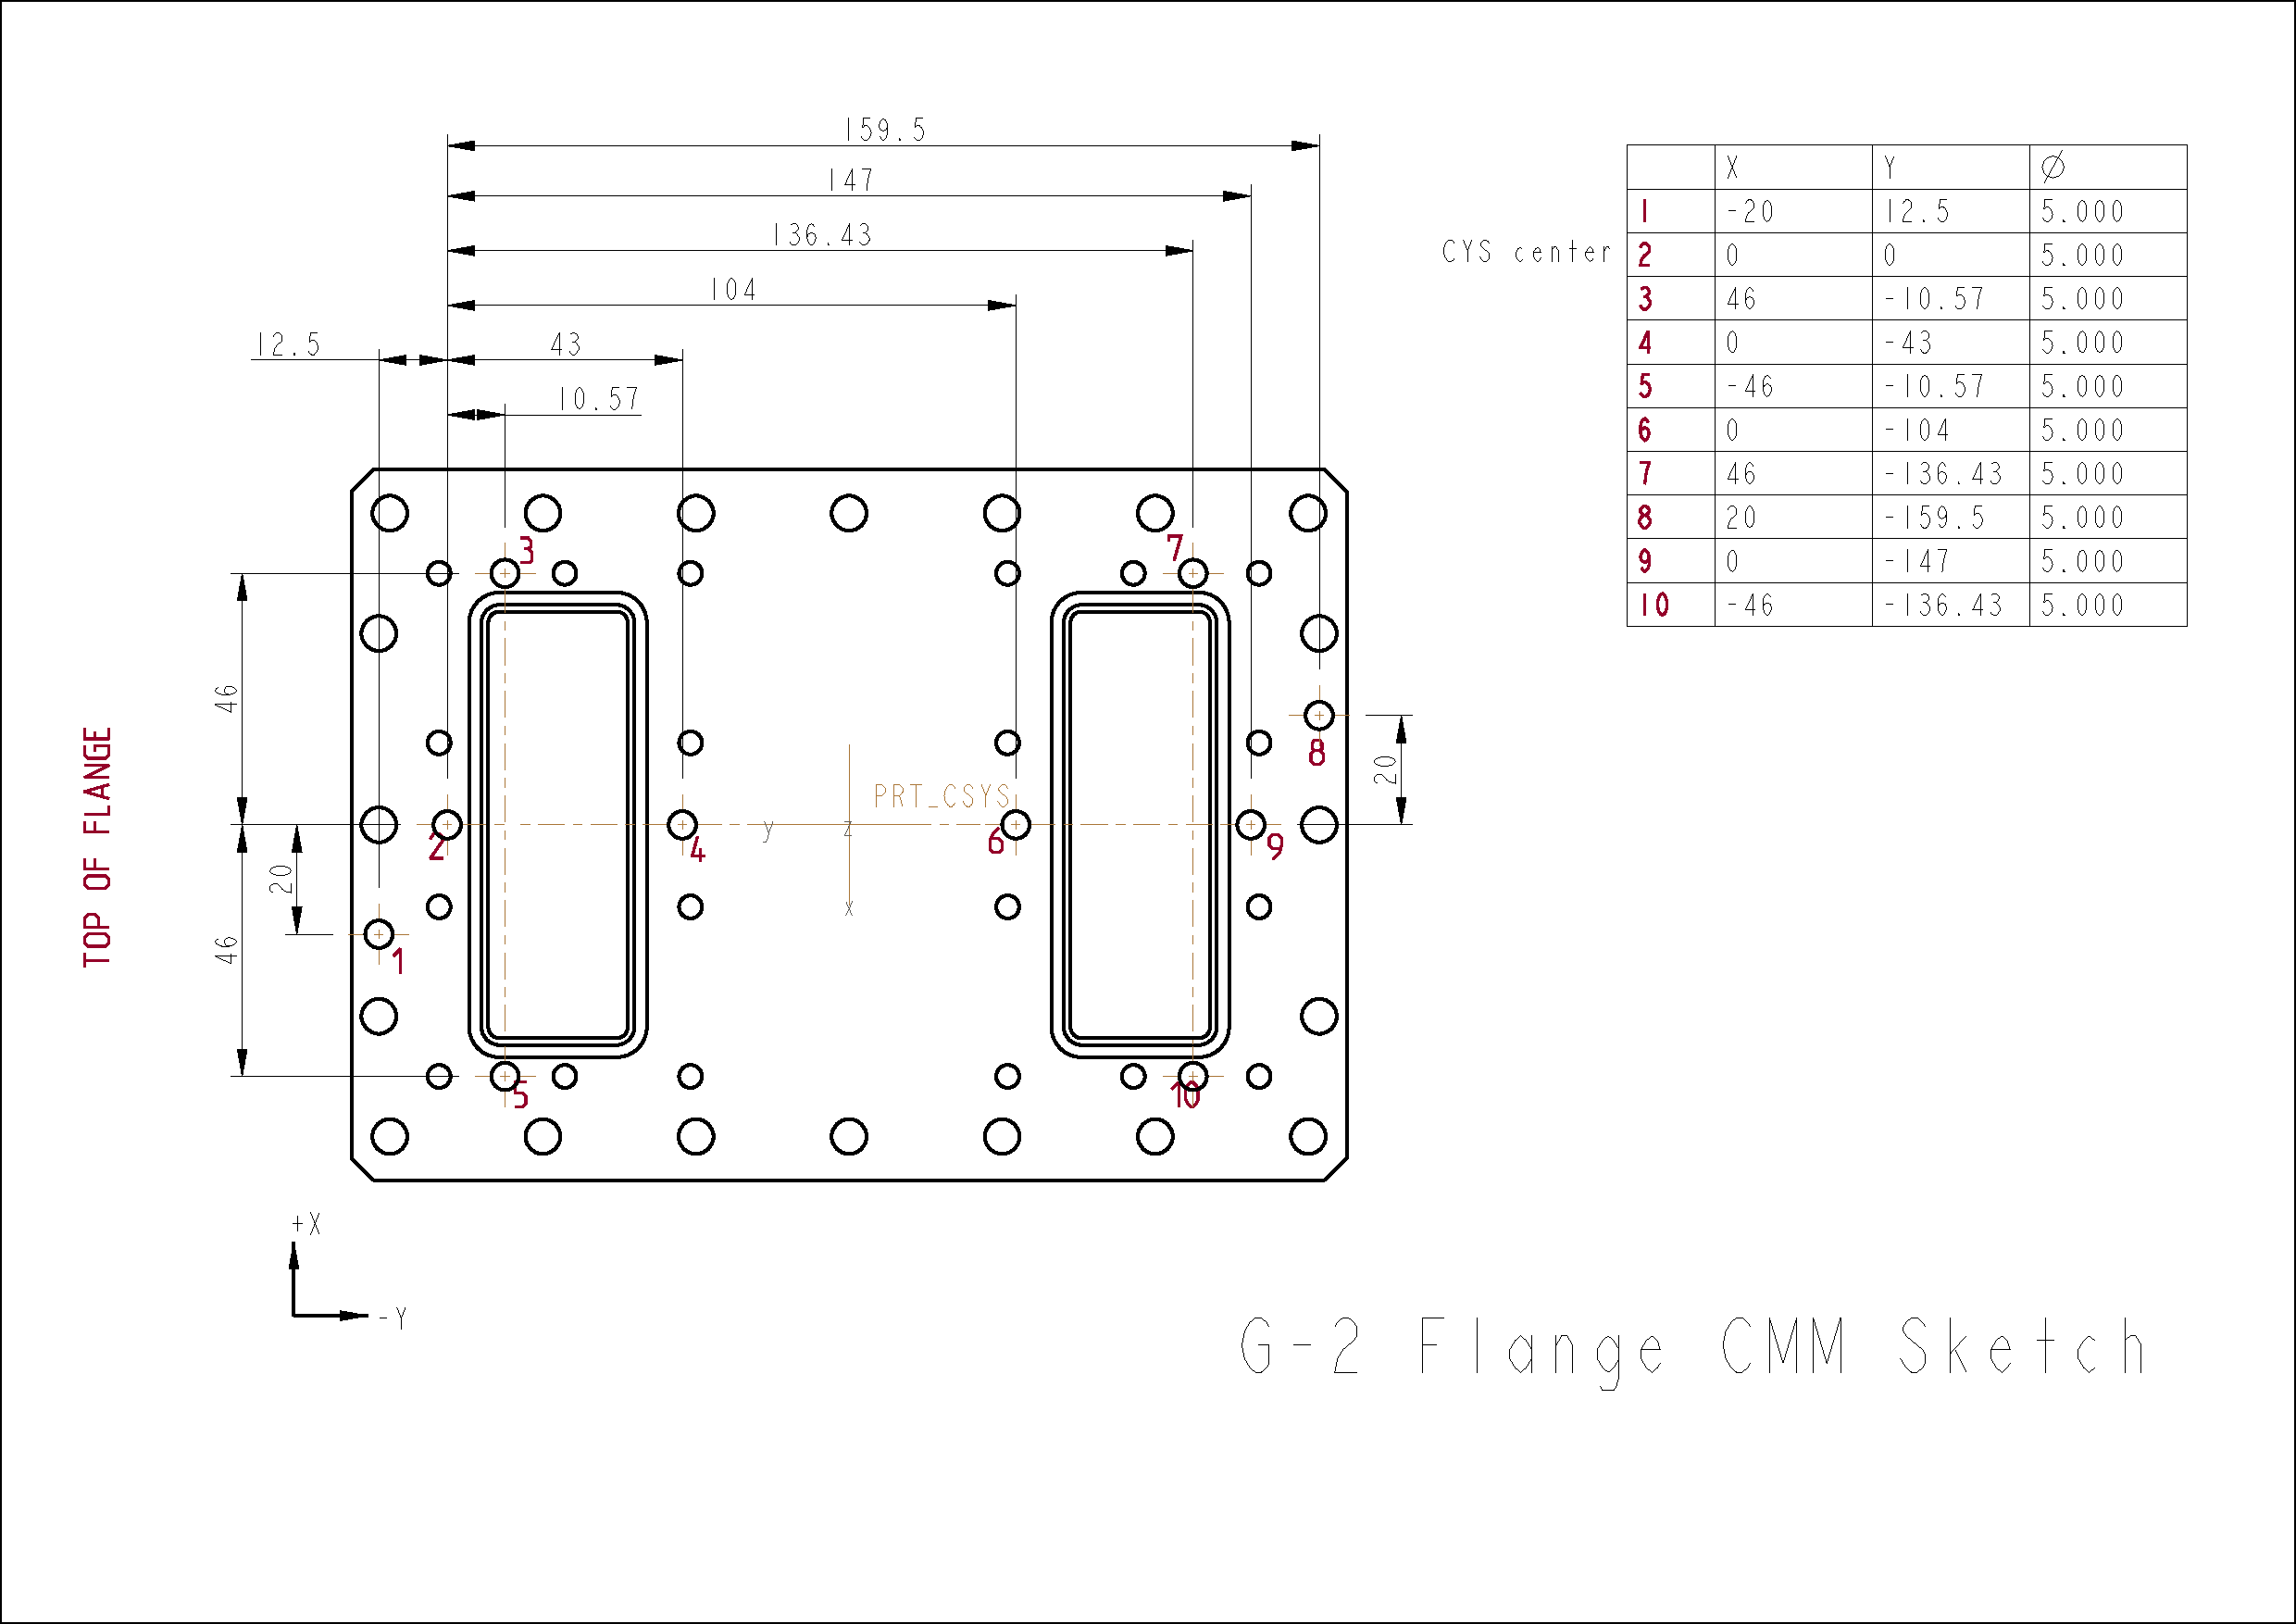
\includegraphics[scale=0.3]{Figures/Flangedrawing.pdf}
\decoRule
\caption{Engineering drawing of the flange with the nominal hole positions and sizes displayed}
\label{fig:Flangedrawing}
\end{figure}

After the manifolds, flanges and lids have been machined the dimensions of various features of the manifold including dowel holes, surfaces and the size and position of each straw hole is precisely measured using a contact probe with a Coordinate Measuring Machine (CMM). The aim is to learn how accurately the parts have been machined and hence to assess if they lie within acceptable tolerances. Therefore determining whether they are ready for use in module construction or need to be returned to the workshop for alteration. An engineering design sheet showing the required hole positions and sizes for the flange is shown in figure 6.6. The dimensions of each piece are required to be known accurately for alignment of the tracking detectors once they are placed into the storage ring. A program was written to measure these points automatically as previously all 1326 points needed for the measurements were done by hand. This improved the measurement time from approximately 6 hours manually to 50 minutes automatically. The manifolds are then paired with a vacuum flange based on the offsets also measured in the flanges. The data is stored in the Liverpool construction database which could then be utilised for any detector alignment studies required.

\begin{figure}[th]
\centering
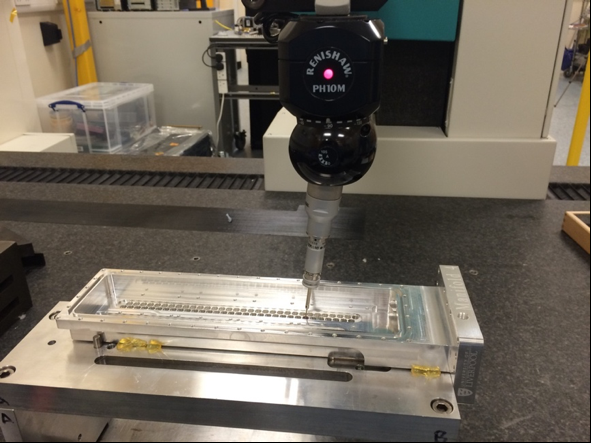
\includegraphics[scale=1.3]{Figures/cmm1}
\decoRule
\caption{Picture of a CMM measurement of the manifold straw holes.}
\label{fig:cmm1}
\end{figure}

The software Metrosoft Quartis \cite{metrosoft} was used to write a program to control the CMM to measure all the parts of the manifold, flange and lid required. This program uses CAD models of the modules pieces to select the elements to assess and the number of probe points required for each measurement. A separate program was written to measure the all three pieces.

The manifold is glued to a stand which is itself fixed in position to the granite work surface of the CMM. This ensures the position of the piece relative to the granite work surface is constant for each separate manifold measurement. Therefore the probe can find the correct position to start its measurement program. The setup is shown in figure 6.7. From this a coordinate system for the stand can be set up and used each time so that the probe will automatically know where it is relative to the manifold. This is done using the 3-2-1 method. Where manually a plane of 3 points is made on the stands face. This is set to a primary direction of z and origin of z. Next a line of two points is measured on the side face of the stand, setting a secondary direction of x and an origin of y. A point is then measured on the other face and set as the origin of x. This was done the first time a program was written, saved and used each time. Next the manifold coordinate system is created with its origin located on a corner of the manifold end. This is done using the 3-2-1 method again. This co-ordinate system is shown in figure 6.8. This coordinate system is saved and will be redone each time a new manifold is measured as there is likely to be a slight deviation in the position compared to the previous manifold measured. This ensures the coordinate system of the CAD is updated to the correct alignment for each metrology measurement. 

\begin{figure}[th]
\centering
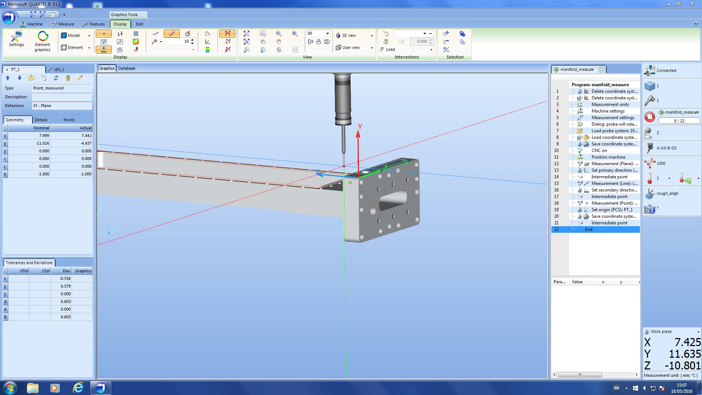
\includegraphics{Figures/cmm2}
\decoRule
\caption{Setup co-ordinate system of the manifold.}
\label{fig:cmm2}
\end{figure}

\begin{figure}[th]
\centering
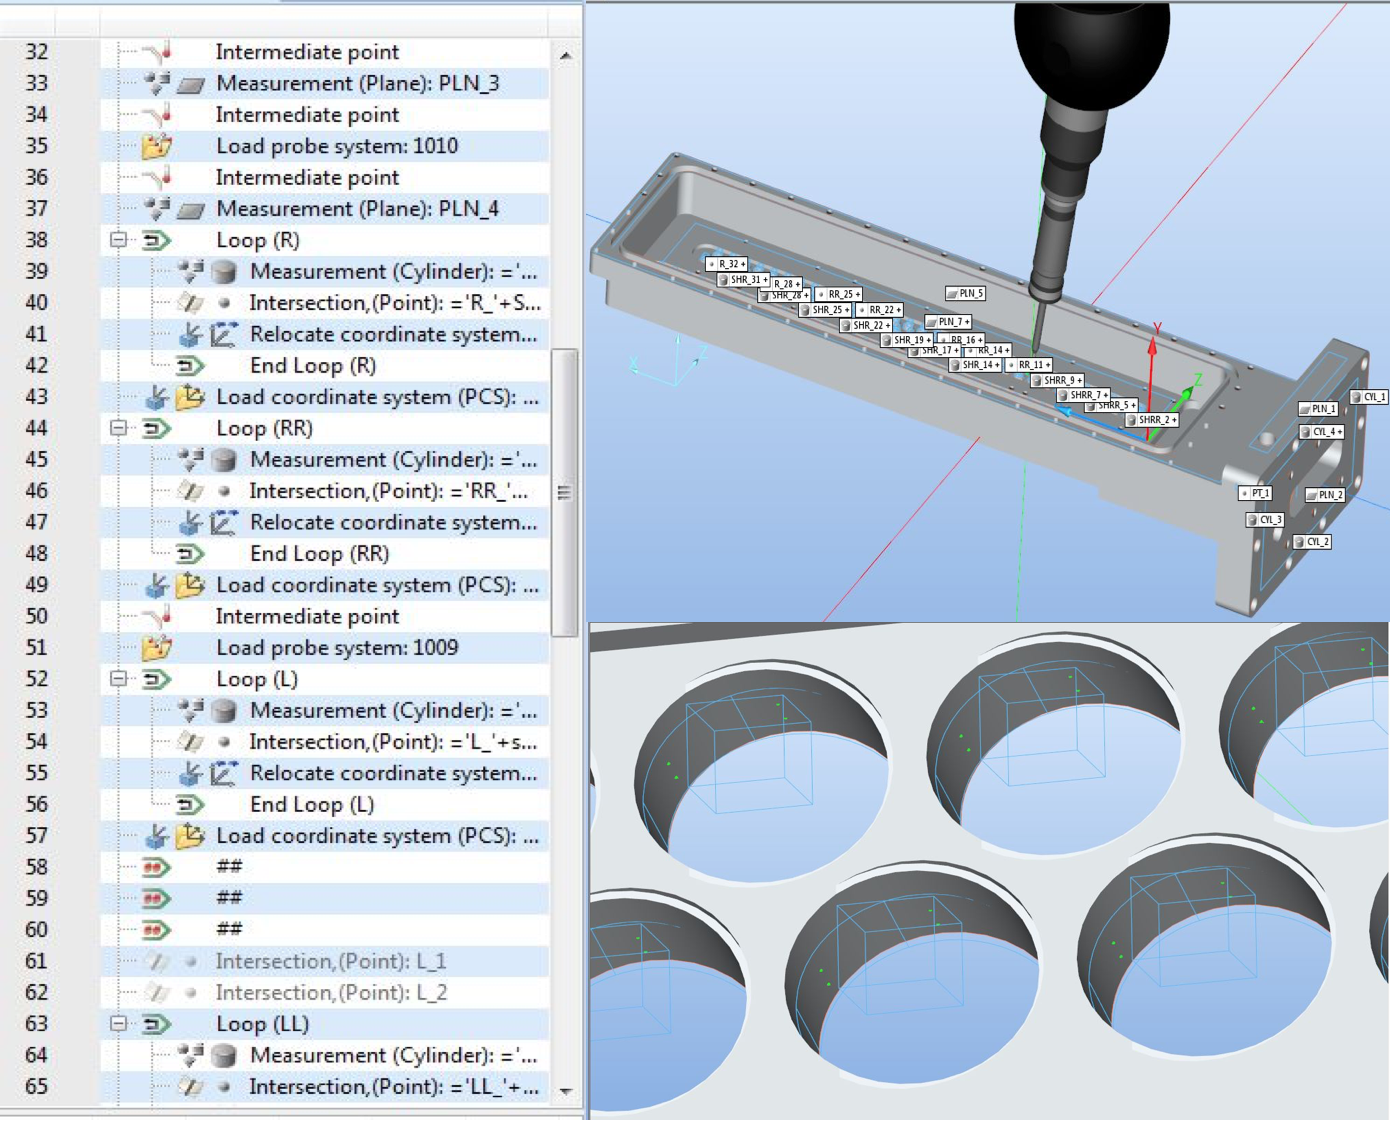
\includegraphics[scale=0.5]{Figures/ccmprogram.png}
\decoRule
\caption{Left: A screenshot of the Metrosoft Quartis program. Right: A screenshot of the program display as the CMM program is running to measure the manifold.}
\label{fig:cmmprogram}
\end{figure}

\begin{figure}[th]
\centering
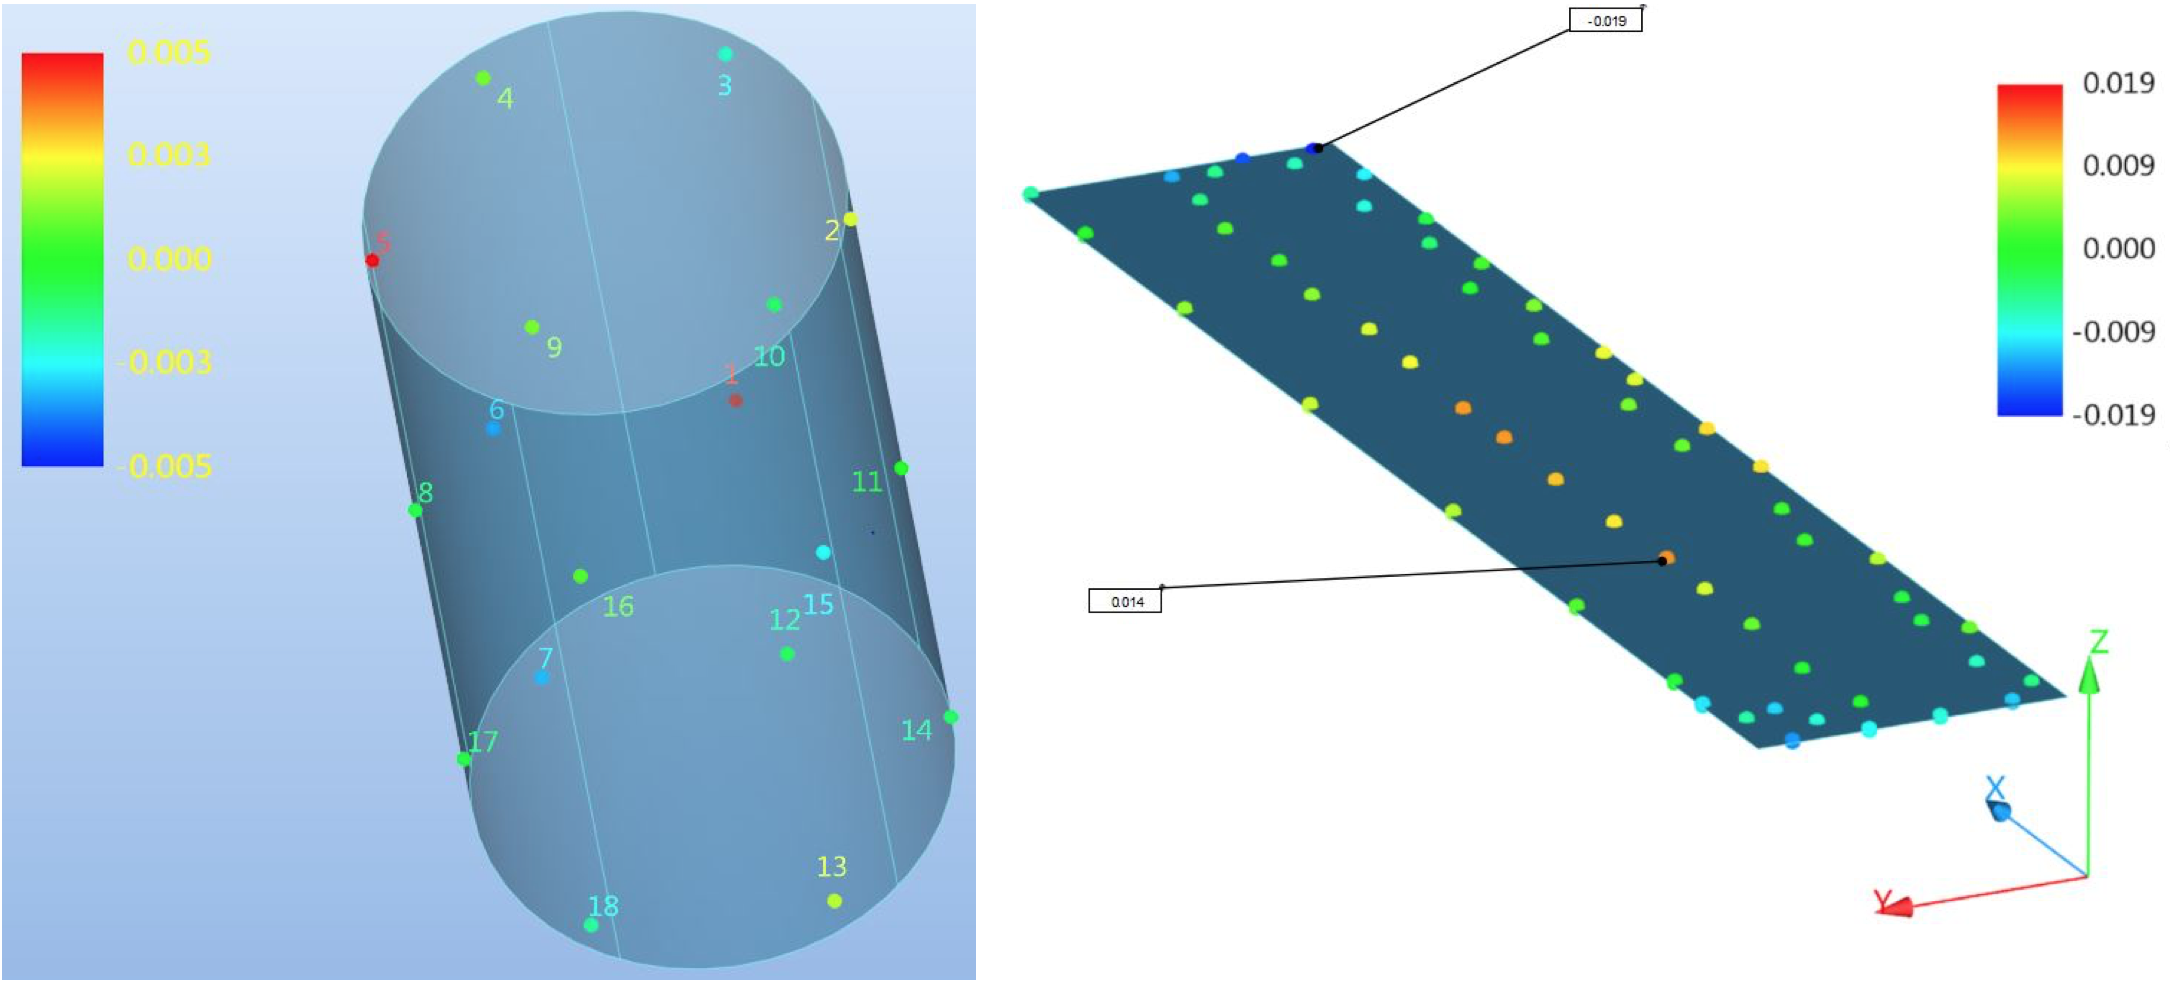
\includegraphics[scale=0.4]{Figures/cmmresults.png}
\decoRule
\caption{Graphical images of results from the Metrosoft Quartis database. Left: A plot of a dowel hole displaying the probes points and their difference from their nominal value. Right: A plot of a plane on the manifold with the probe points showing their difference from the nominal flatness in mm.}
\label{fig:cmmresults}
\end{figure}

At the start of a new set of measurements the probe dimensions needed to be calibrated manually using the reference sphere. The dowel holes and 128 straws holes of the manifold are required to be known in size and position precisely. These were measured as cylinders by the probe which could also determine if there were any bumps inside the holes which would need to be removed. The programming of the measurement of the dowel holes and straw holes is shown in figure 6.9. The straw hole measurements were carried out by a program using a loop which measures a cylinder and moves the probe 6.052 mm along to the centre of the neighbouring hole. This was done for each straw row. As the expected positions are given in the CAD model any deviations of individual holes or offsets of entire rows will be measured by the probe. Along with the holes, the various manifold faces and O-ring plane were also measured for flatness, tilting and positioning.

Once all measurements are completed, the database contains all the values required including nominal values, the values measured and the range of measurements for each element. From this data any alterations to the pieces of equipment can be carried out. The data is then used to match pairs of manifolds together with similar offsets and chose a flange to match with the manifolds. Plots from the database showing a cylinder from a dowel hole measurement and a surface element from a manifold surface displaying the measured probe points deviation from the nominal values are shown in figure 6.10. Plots showing the straw holes and flange dowel holes measured are shown in figures 6.11 and 6.12 respectively.
%put in a histogram of the hole sizes (difference from nominal) and positions (difference from nominal)

\begin{figure}[!h]
\centering 
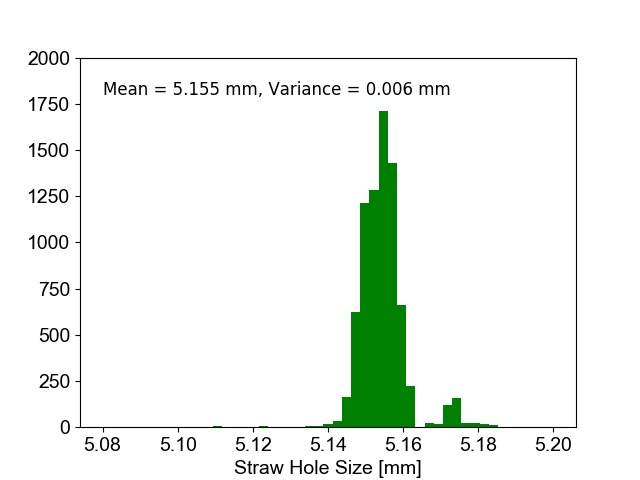
\includegraphics[scale=0.6]{Figures/strawholesizes.jpeg}
\decoRule
\caption{Plot displaying the measured manifold straw hole sizes for all manifolds measured. The nominal size for a straw hole being 5.15$\pm0.2$ mm. }
\label{fig:strawholesizes}
\end{figure}

\begin{figure}[!h]
\centering 
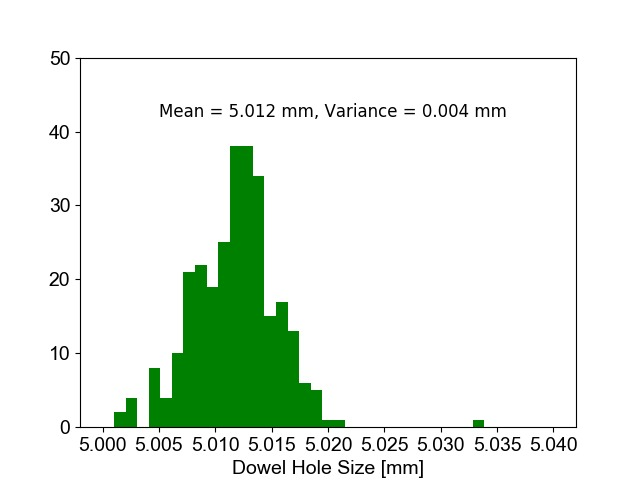
\includegraphics[scale=0.6]{Figures/dowelholesizes.jpeg}
\decoRule
\caption{Plot showing the size of all flange dowel holes measured. The nominal size for a flange dowel hole is 5.0$\pm0.2$ mm.}
\label{fig:dowelholesizes}
\end{figure}

\section{Preparation of wires (Wire crimping and threading)}

The wires are prepared prior to being strung into the manifold. This involves threading the wire through gold plated Copper pins. The 25 $\mu$m gold plated Tungsten wire is threaded through a long pin which is then crimped using the materials tester to secure the wire in place. The copper wire must be cut to a length longer than the straw module, so lengths of about 80cm were cut. The wire is threaded through the injection molded insert which contain slots to allow gas flow through the straws and secondly through a long pin. Glue is then applied to the end of the long pin which is then placed inside the insert, leaving a small length of the wire going through the pin with most left behind the insert. 

To secure the wire in place the long pins are crimped using a Lloyd LRX Plus materials tester \cite{LloydPlus}. The pins are placed horizontally into the materials tester to ensure an even distribution and are crushed using a 1kN load cell. A photograph of the crushing process is shown in figure 6.13 with a close up photograph shown in figure 6.14. To measure this process a Epsilon Extensionometer \cite{Extensionometer} is attached to the crushing jaws to measure its extension as it crushes the pin. This data produces a graph which is checked to ensure that the crimping was carried out correctly, along with the measurement of the pins diameter before and after crimping.

The wires are then left for 24 hours to allow for any expansion of the pin after the crimping process. The short length of the wire is then gently pulled while holding the insert to see if the wire can be pulled through and hence the crimp has failed. Any wires that fail this will be re-crimped and pull tested again. 

\begin{figure}[!h]
\centering 
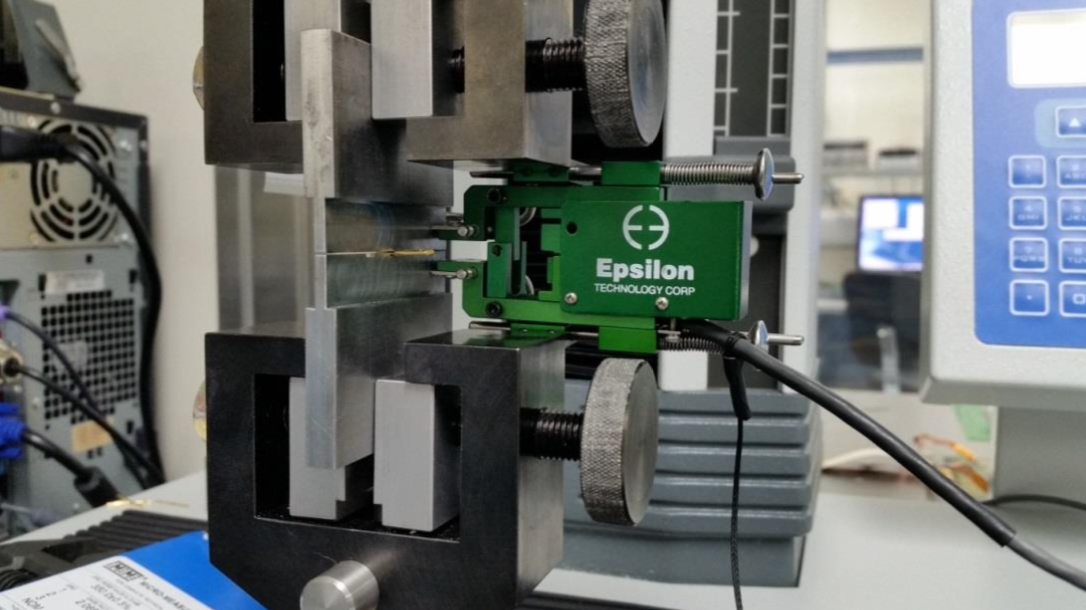
\includegraphics[scale=0.75]{Figures/crimpmachine}
\decoRule
\caption{Photograph of the Lloyd LRXPlus materials tester crimping a pin.}
\label{fig:crimpmachine}
\end{figure}

\begin{figure}[!h]
\centering 
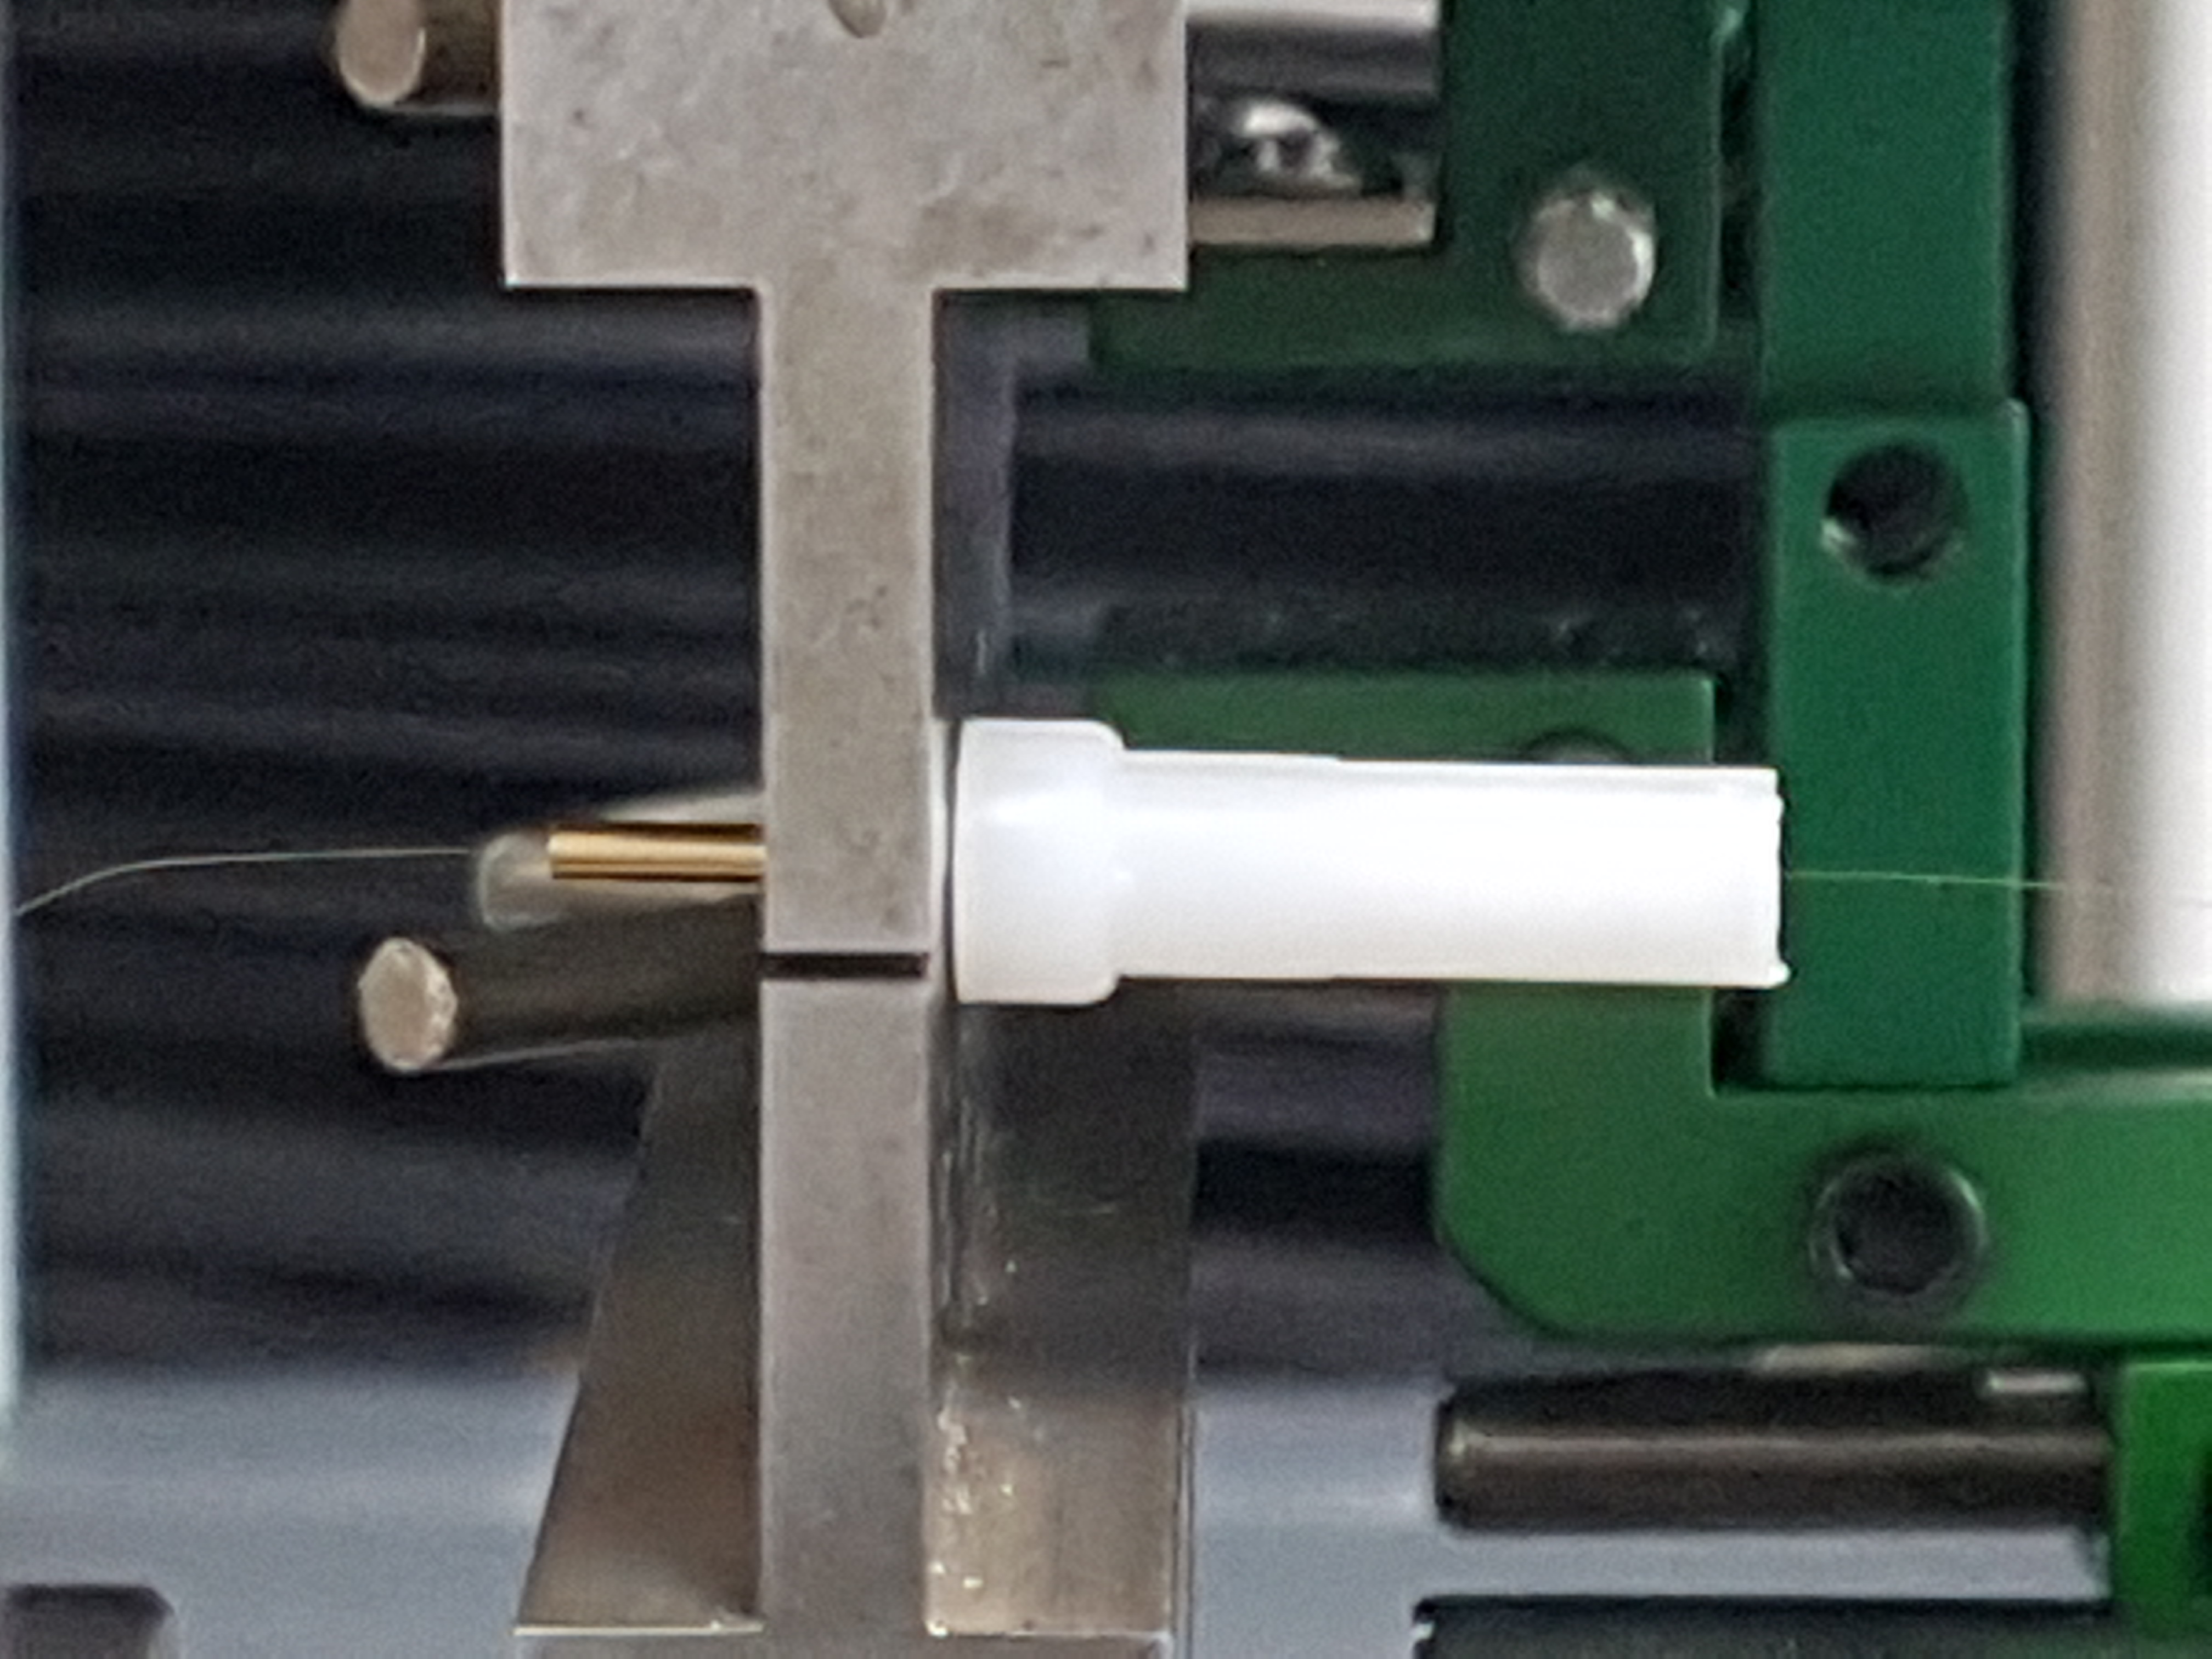
\includegraphics[scale=0.08]{Figures/pincrush.jpg}
\decoRule
\caption{Close up photograph of a pin being crushed.}
\label{fig:pincrush}
\end{figure}

\section{Straw assembly}
The long straws that have passed leak and resistance tests are then cut into 90.6 mm sections with a guillotine. This usually makes 12 shorter straws. The top hat and non-top hat end pieces are then glued to each end of the straw. This is done using a Q-tip to carefully apply a silver epoxy TraDuct 2902 \cite{silverepoxy} to the end pieces and attach them to the straw ends ensuring that the straws are not bent or damaged as the two are bonded together. A row of completed straws is shown in figure 6.15.

\begin{figure}[!h]
\centering 
\includegraphics[scale=0.05]{Figures/completestraws.jpg}
\decoRule
\caption{Photograph of a row of 32 completed straws.}
\label{fig:completestraws}
\end{figure}

The selected manifold pair plus the flange are put together, positioned correctly and then secured in place by jacks which hold the manifolds a selected distance apart. Then the module is potted with 128 straws. In total the process to glue 128 straws into the module takes 5 days. Firstly the straws have silver epoxy applied between the straw and module. This is used to produce an electrical grounding of the straw to the module. To provide a gas seal between the straw and the module Araldite 2020 is also applied. The process requires 5 days due to the time that the curing takes to dry and the fact that only one layer is done at a time to minimise the risks of moving or knocking the straws while the bond is curing.

\section{Module construction}

The modules are placed on the stringing jig which is used to populate the straws with the individual wires. The prepared wire is threaded through a straw using a plastic rod with a hole in the end to attach the wire. This will be pulled the entire way through a straw to the opposite end and removed from the other side to thread the wire. A photograph of this is shown in figure 6.16. The end with the pre-crimped pin goes into the top hat side of the straw and is fixed there while the bare end of the wire is pulled through to the other end of the straw. Another insert is threaded through the wire and fixed into the non-top hat end, with a short annealed pin being threaded onto the wire. The short pin is annealed so that it is easier to crimp with a hand tool. Once both the insert and pin are threaded through the wire a 30 g weight is hung from the end of the wire to provide the required tension while the pin and insert are being secured into the module and until the wire has been crimped and fixed in place. The short pin is then glued into the insert and then the pin is crimped with a hand crimp tool to secure the wire in place. The remaining wire with the weight attached is then cut off and the wire trimmed off as close as possible to the pin end. Glue is then placed on top of the wire to cover it and stop any electrical discharge that could occur. The stringing process is repeated for all 128 straws. Once the stringing process has been completed, the jacks that are holding the manifolds in place are moved apart 50$\mu$m to produce a 50 g tension equally to the straws and wires. This is done to compensate for expansion under vacuum.
\begin{figure}[!h]
\centering
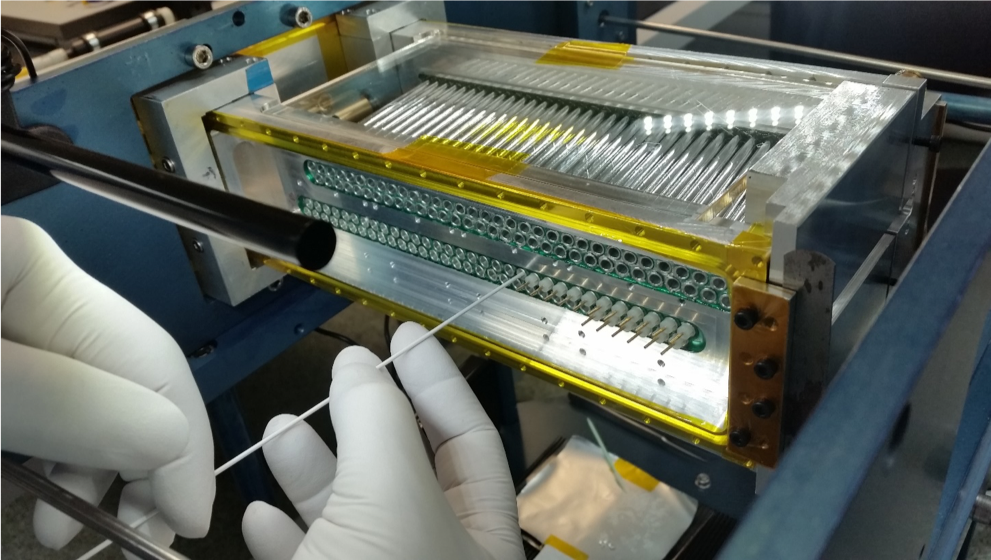
\includegraphics[scale=0.85]{Figures/string}
\decoRule
\caption{Photograph of a wire being threaded into a straw on the stringing jig.}
\label{fig:string}
\end{figure}

\section{Post module assembly wire testing}

The wires are required to have a tension test after stretching to ensure that no wire failures have occurred. A tension within 25-50g is required, preferably the wires being closer to 50g. This is about half of the tension needed to break a wire. The higher tensions are desirable to minimise the gravitational sag on the wires.

The tension test is carried out by placing a magnet above the test straw. This is positioned above the straw onto a thin layer of perspex to protect the straws. Then a crocodile clip is attached to each end of the straw pins. The tension is measured by sending current down the wire and varying its frequency in an external magnetic field. The varying electric field will make a magnetic field and the wire will resonate in the external magnetic field. The current of the wire is recorded after every pulse. When the frequency of the current pulse reaches the resonance frequency of the wire, the current induced in the wire will be recorded and used to calculate the tension. A photograph of a tension test is shown in figure 6.17.

The tension tester calculates the wire tension using the equation: 
\begin{equation}
f=\frac{\sqrt[2]{\frac{T}{\frac{m}{L}}}}{2L}
\end{equation}
where f is the frequency in Hertz, T is the tension in Newtons, m is the mass of the wire in kilograms and L is the length of the wire in metres. 

\begin{figure}[!h]
\centering 
\includegraphics[scale=0.08]{Figures/wiretesting.jpg}
\decoRule
\caption{Photograph of a tension test being carried out on a wire.}
\label{fig:wiretesting}
\end{figure}

A resistance test is also carried out on each wire. This is done by touching probes to the pins on either end of the wire which are connected to a digital multimeter. The resistance of each wire should be within the range of 10 - 13 $\Omega$. If wires lie outside this range, they will be removed and re-strung. A carbon fibre post is then fitted the non flange end of the module and used to keep the manifolds in position. The new manifold separation distance is checked using the CMM, and then the jacks can be removed.

\section{Module electronics installation}

Once the resistance and tension tests have been completed with any re-stringing done and the wires have passed all requirements the modules electronics can be inserted. The electronics required include eight ASDQ boards (four per manifold) which are placed onto readout long pins. End caps are placed onto the short pins providing insulation to stop any electrical discharge from the pin to the ASDQ boards. The two ASDQ chips on each board are then covered with a PTFE thermal heat pad. This is to prevent the boards overheating by transferring the heat to Copper heat sinks which are fixed to the ASDQ boards using brass screws. The heat sinks pass the heat onto the manifold. Four flexi cables and HV cables are connected to the feedthrough board and inserted through the Snout and connected to the relevant ASDQ boards. A photograph of this is shown in figure 6.18. The feedthrough board is then fixed to the Snout and sealed up to provide a gas seal. Finally the o-ring is covered in vacuum grease, put in place then the lid is secured in position with a torque wrench to seal the lid to the manifold and ensure the lid is attached evenly.

\begin{figure}[!h]
\centering
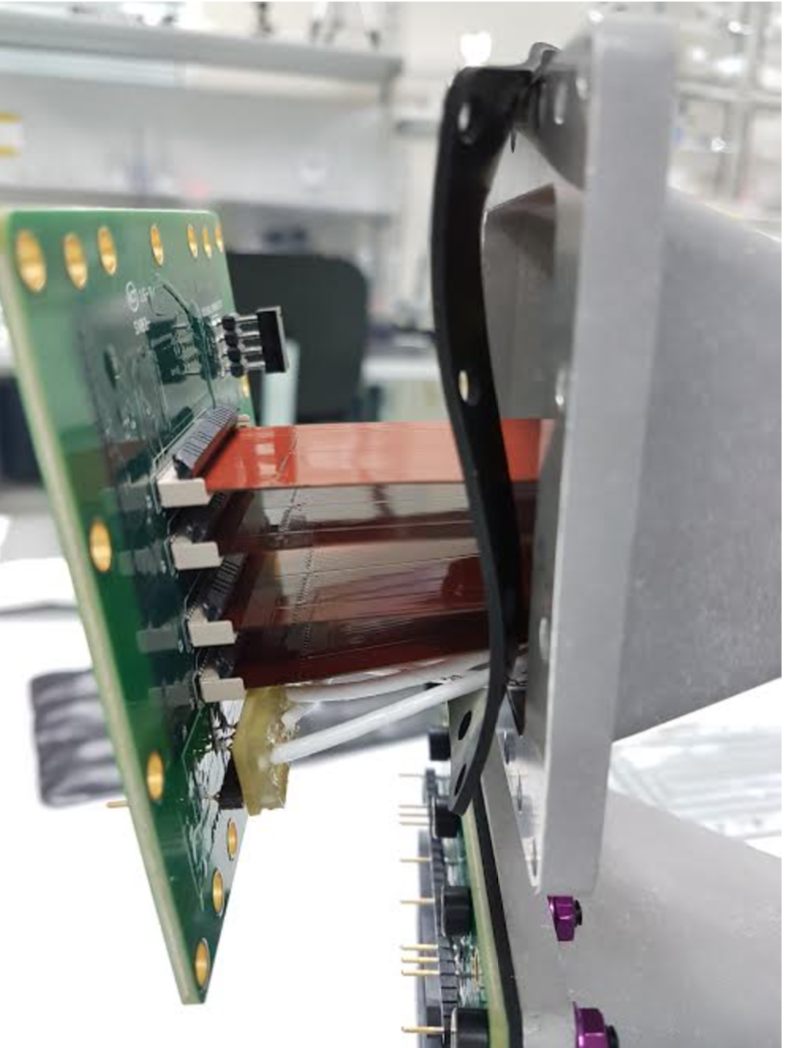
\includegraphics[scale=0.4]{Figures/flexicables}
\decoRule
\caption{Photograph of flexi cables and HV internal cables connected to the feedthrough board at Snout end of the module.}
\label{fig:flexicables}
\end{figure}

\section{Module Checks and Data Quality}

Before the constructed modules can be shipped to Fermilab, several tests must be carried out to ensure that the module can run at a sufficient vacuum, all wires are recording hits correctly and that the module can run at the required high voltage for a sufficient amount of time. These tests are done by placing the module horizontally into a vacuum chamber to provide the maximum number of cosmic hits for data taking. The module is bolted into the vacuum tank and vacuum sealed using a greased O-ring. The 80:20 Ar:$CO_2$ test gas is flowed through the module at a rate of 0.1LPM into the top manifold, out through the bottom manifold and directed into a bubbler. This is used to check the gas flow. A photograph of the setup is shown in figure 6.19.

\begin{figure}[!h]
\centering
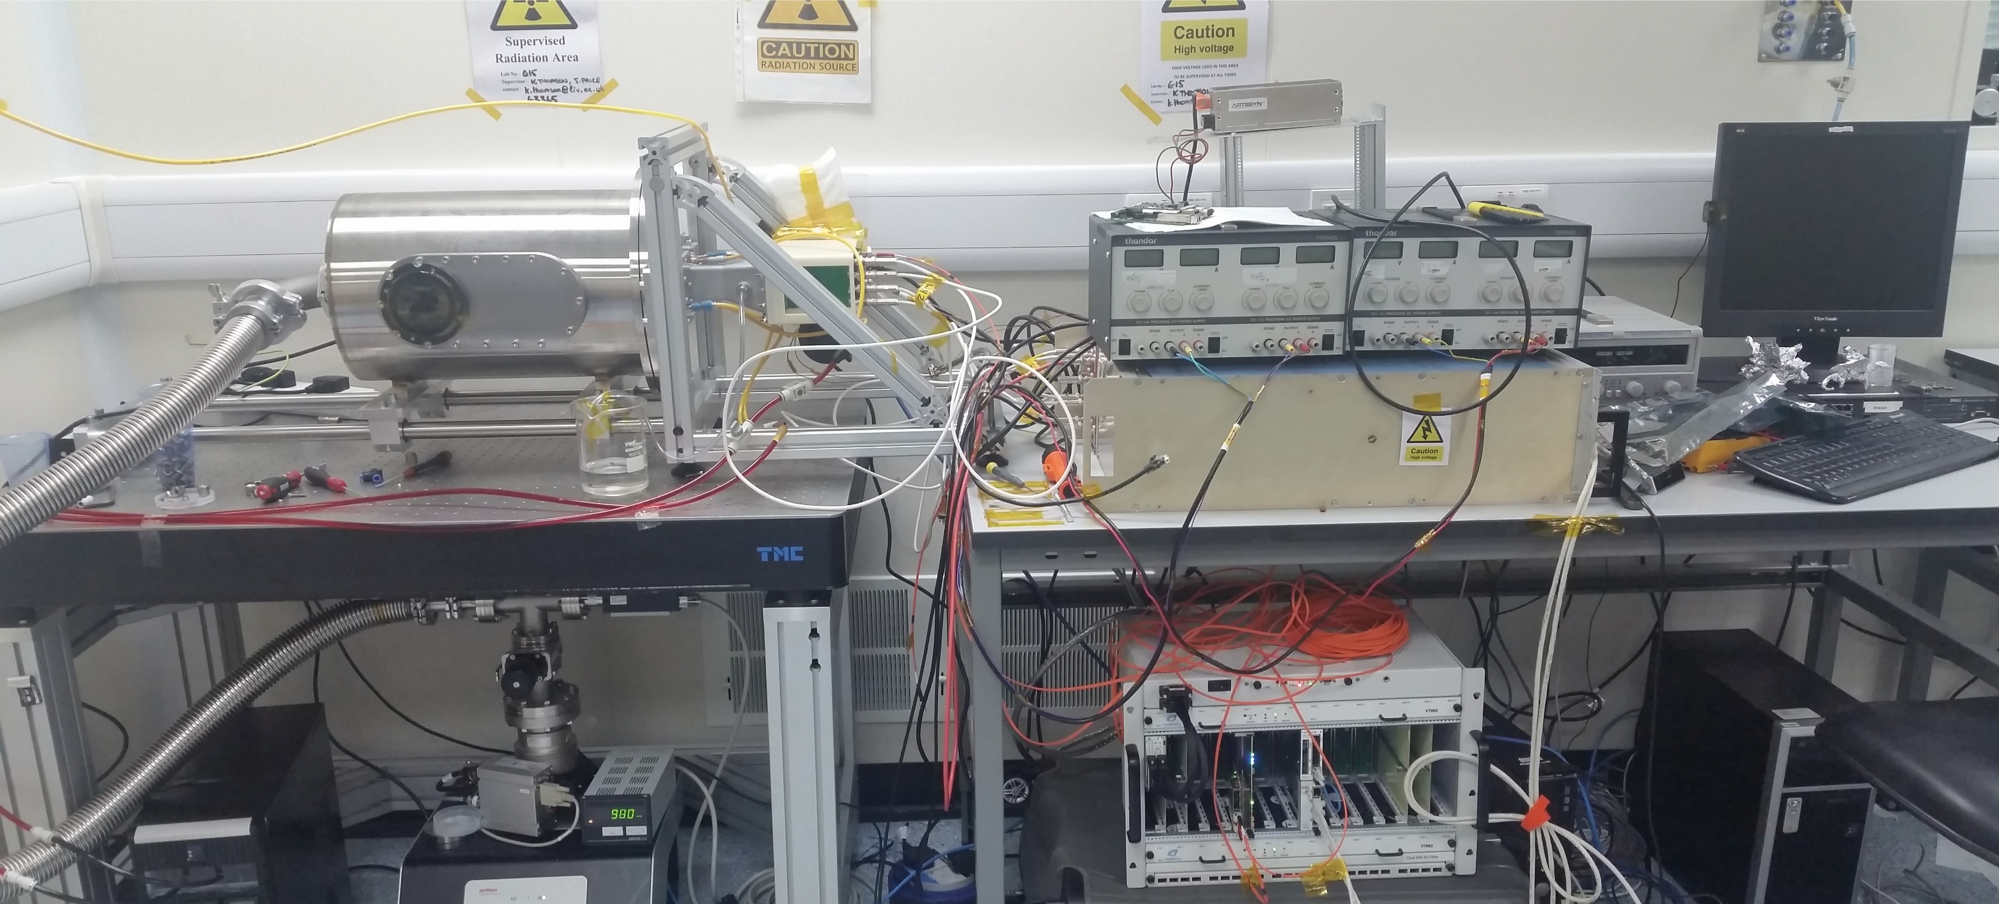
\includegraphics[scale=0.4]{Figures/DAQsetup1}
\decoRule
\caption{Clean room setup for module testing including the vacuum tank for vacuum testing on the left and CAEN power supply on the right.}
\label{fig:DAQsetup1}
\end{figure}

\subsection{Vacuum testing}

The vacumm pump down begins with a roughing pump which takes it down to 10 mbar. Then the turbo pump is needed to lower the pressure to the order of $10^{-6}$ mbar as required for the experiment. This data is continually monitored as shown in figure 6.20. If the module pressure struggles to get below $10^{-3}$ mbar after one day of pumping, this indicates that the module has a leak that needs to be investigated. The vacuum will be monitored to ensure that the pressure can stay to the required level for significant amount of time.
\begin{figure}[!h]
\centering
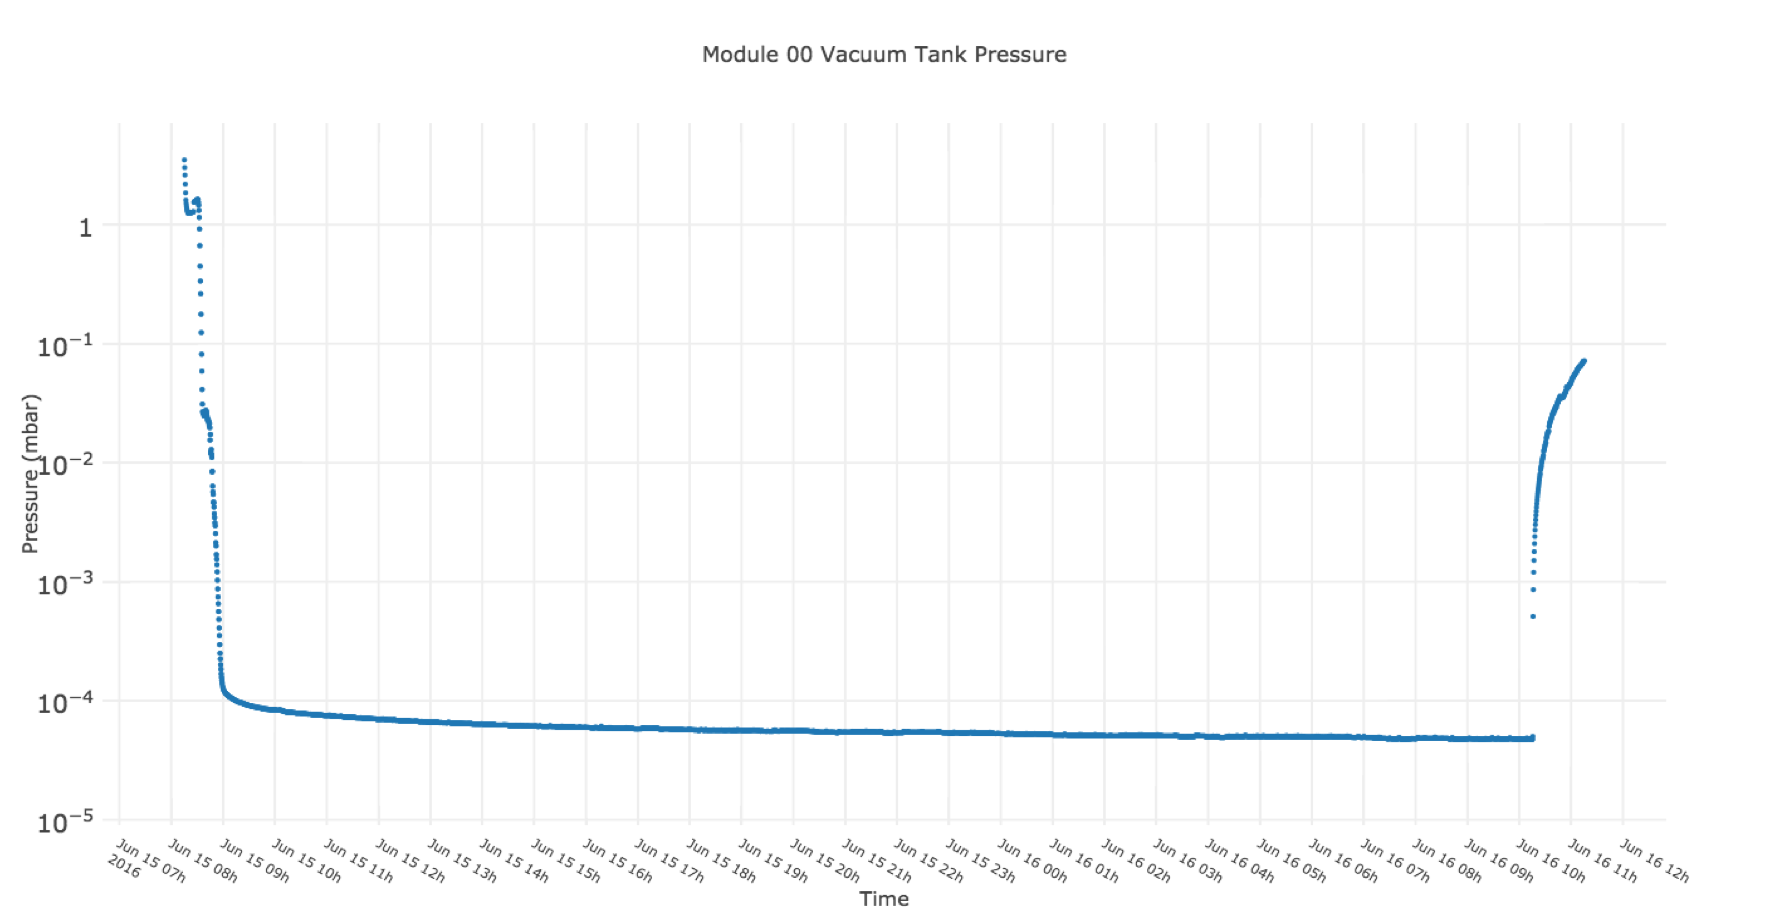
\includegraphics[scale=0.4]{Figures/vactankpressure}
\decoRule
\caption{Graph of a successful module pump down, with rapid pump down on the left and vacuum shut down on the right.}
\label{fig:vactankpressure}
\end{figure}

\subsection{ High and low voltage noise scans}

Once the required vacuum level has been maintained the Front End Electrons as explained in chapter 5 are placed into a custom made box which is fixed to the Snout. Low and high voltage noise scans will be carried out to ensure that no residual noise from the wires is observed above the 200mV threshold. This also checks if all the connections to the internal electronics are working, with the 16 channels per ASDQ board all recording data. If channels are not working this could indicate a shorted connection, a broken wire or problems with the HV connection. The threshold was set at 200mV as this was deemed high enough to cover most of the residual noise from the wires whilst not losing too many low energy straw hit signals. For noise scans every channel is tested at three voltages of 1000V, 1250V and the near-operating voltage of 1500V. The actual voltage in the experiment is 1650V, but Ar:$CO_2$ breaksdown at this value, and could contaminate the wires. If working correctly all the channels at all voltages should be working identically. A plot of an ASDQ that passed a noise scan is shown in figure 6.21. For channels that do not work, this would show that the wire connection is faulty or that the wire has a contaminant. Once 1500V has been successfully reached, this is left for a day to test if it runs stably. If a failure is observed and it is suspected to be due to a wire contaminant then high voltage training is carried out. To do this the HV is increased in increments of 100 V from zero until the channel trips. Then the trip current is increased from 1$\mu$A to 3$\mu$A and left at this current for a couple of hours to remove the contaminant.

\begin{figure}[ht!]
\centering
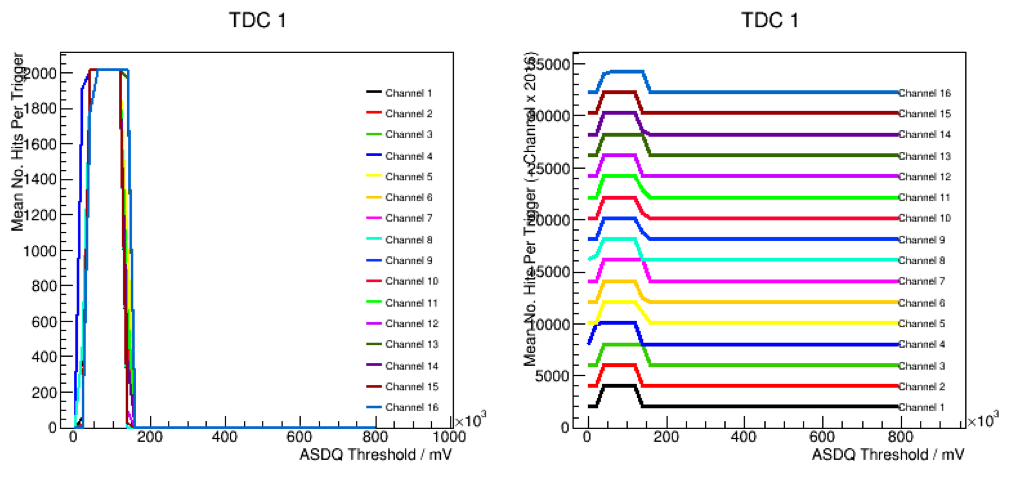
\includegraphics[scale=0.8]{Figures/HighVNoiseScans}
\decoRule
\caption{Example plot of a High voltage noise scan that has passed testing.}
\label{fig:HighVNoiseScans}
\end{figure}

\subsection{ Module testing using cosmic muon data}

Once all testing has been completed and the vacuum and HV are running stably then DAQ runs with muon cosmic data are taken. A four hour test, which is the minimum time required to detect hits in all 128 channels, was carried out. If a channel had zero hits in this time it indicates a dead channel. Once any dead channels have been fixed much longer cosmic data runs were carried out. This was to ensure that the module could record data stably for a significant amount of time. Plots of a long cosmic run are shown in figures 6.22 and 6.23 displaying the hits recorded in all four rows of straws.

\begin{figure}[th]
\centering
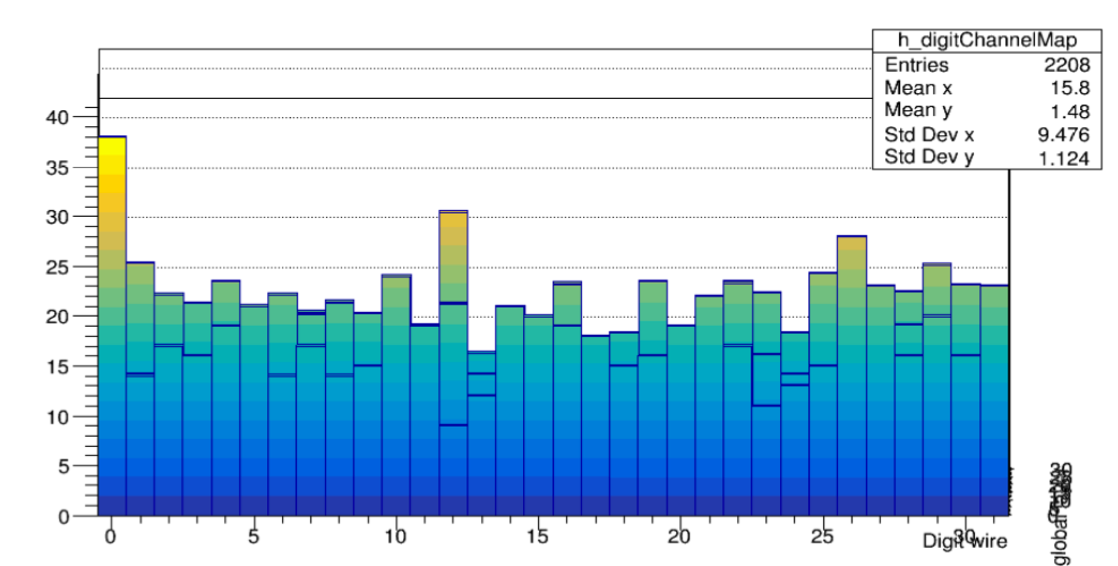
\includegraphics[scale=0.75]{Figures/cosmicdata1}
\decoRule
\caption{A plot of cosmic data channel hits for the four rows of straws.}
\label{fig:cosmicdata1}
\end{figure}

\begin{figure}[th]
\centering
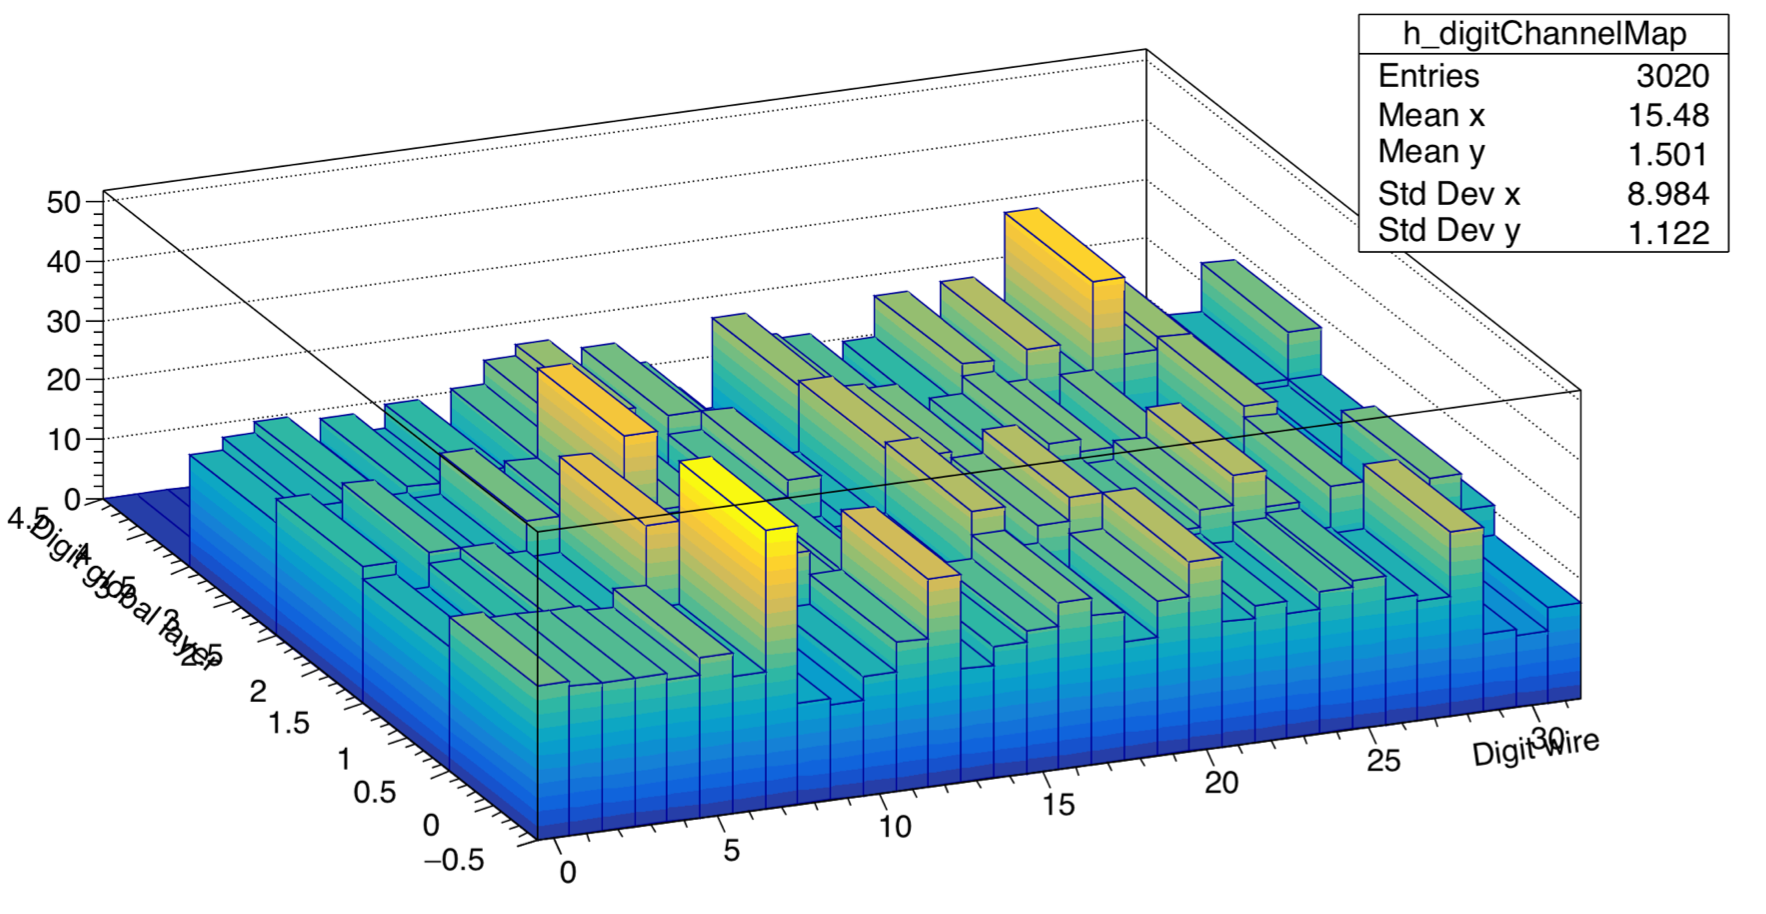
\includegraphics[scale=0.4]{Figures/cosmic4rows.png}
\decoRule
\caption{A 3D plot showing more clearly the cosmic data channel hits for the four rows of straws.}
\label{fig:cosmic4rows}
\end{figure}

Once it has been established that the module has passed all quality assurance testing the module is readied for shipping to Fermilab. This involves covering the module with perspex shielding and an antistatic plastic covering before being placed into a pelicase.


